\section{Epistemic uncertainty}

The second analysis is about the epistemic uncertainty. While this form of uncertainty pertains to the model itself rather than the input data, we want to investigate this aspect. Epistemic uncertainty is computed as:

\[
	epistemic = diag\{\frac{1}{T} \sum_{t=1}^{T} [\hat{p}_t - \bar{p}]^{\otimes 2}\}
\]

In this context, establishing an explicit upper limit for the uncertainty is not an easy task like in the previous case. Conversely, the lower limit is unequivocally $0$, given the inherent non-negative nature of the quantities. Hence, a series of empirical experiments were conducted to find a reasonable threshold range. The outcome determined an upper limit of $0.02$, since values surpassing this upper limit exhibited the same accuracy, indicating that the behavior is that same. As previously, the threshold is calculated through the formula:

\[
	threshold = 0.02 * (1 - conf \_ level), \ with \ con \_ level \in [0,1]
\]

The outcomes of the conducted experiments are visually shown in \Fig~\ref{fig:epistemic_class}, offering different insights into this scenario.

In \Fig~\ref{fig:epistemic_acc}, the shift in accuracy corresponding to decreasing thresholds is showcased. As anticipated, an absence of confidence ($conf_level = 0$) yields an accuracy approximately aligning with the nominal value. Conversely, a complete confidence level ($1$) results in an accuracy raises to $100\%$, attributed to the fact that all predictions are discarded as unknown. This phenomenon is highlighted further in \Fig~\ref{fig:epistemic_unk}, which delineates the trajectory of unknown values. Indeed, with a confidence level set to $1$, the proportion of unknown values escalates to $100\%$, effectively indicating the inefficacy of the predictions.

\begin{figure}[h]
	\centering
	\begin{subfigure}{.5\textwidth}
		\centering
		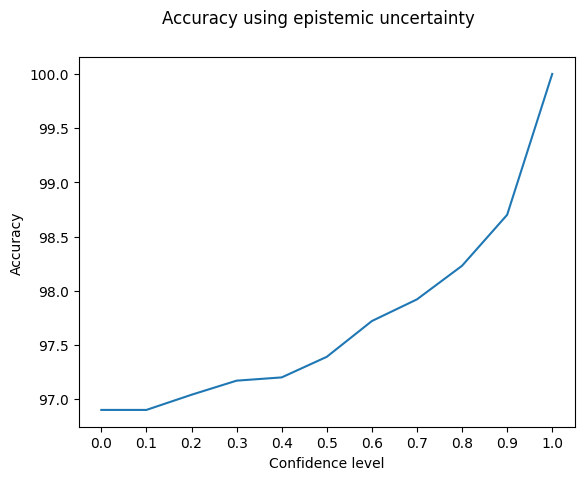
\includegraphics[width=0.8\linewidth]{ImageFiles/ClassifUncer/epistemic_acc}
		\caption{Accuracy trend when the confidence level is increased}
		\label{fig:epistemic_acc}
	\end{subfigure}%
	\begin{subfigure}{.5\textwidth}
		\centering
		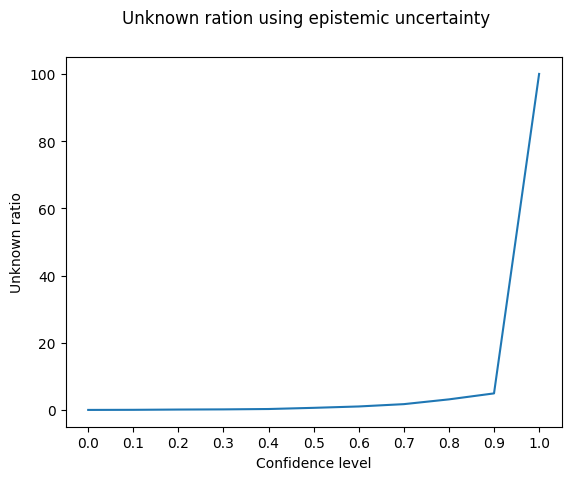
\includegraphics[width=0.8\linewidth]{ImageFiles/ClassifUncer/epistemic_unk}
		\caption{Unknown ratio trend when the confidence level is increased}
		\label{fig:epistemic_unk}
	\end{subfigure}
	\caption{Performances of the BNN using the epistemic uncertainty during classification}
	\label{fig:epistemic_class}
\end{figure}

An interesting fact worth to highlight here is the smoother incremental pattern observed in the accuracy progression. Specifically, as shown in \Fig~\ref{fig:epistemic_acc}, the accuracy gradually ascends to approximately $98.5\%$ at a confidence level of $0.9$, before making a jump to the trivial case of perfect accuracy ($100\%$) at full confidence ($1$). It is noteworthy that in the previous instance, the highest achievable accuracy was around $99.0\%$. While the difference may not be substantial, it implies an underlying distinction that might be hidden due to the already elevated accuracy values. A more comprehensive exploration of the efficacy of these approaches will be conducted later in this study.